%##########################################################################################################################################################################
% Implimentations
%##########################################################################################################################################################################

\chapter{Implementation}
    \section{Overview}
    \begin{minipage}{1\textwidth}
        \begin{center}
            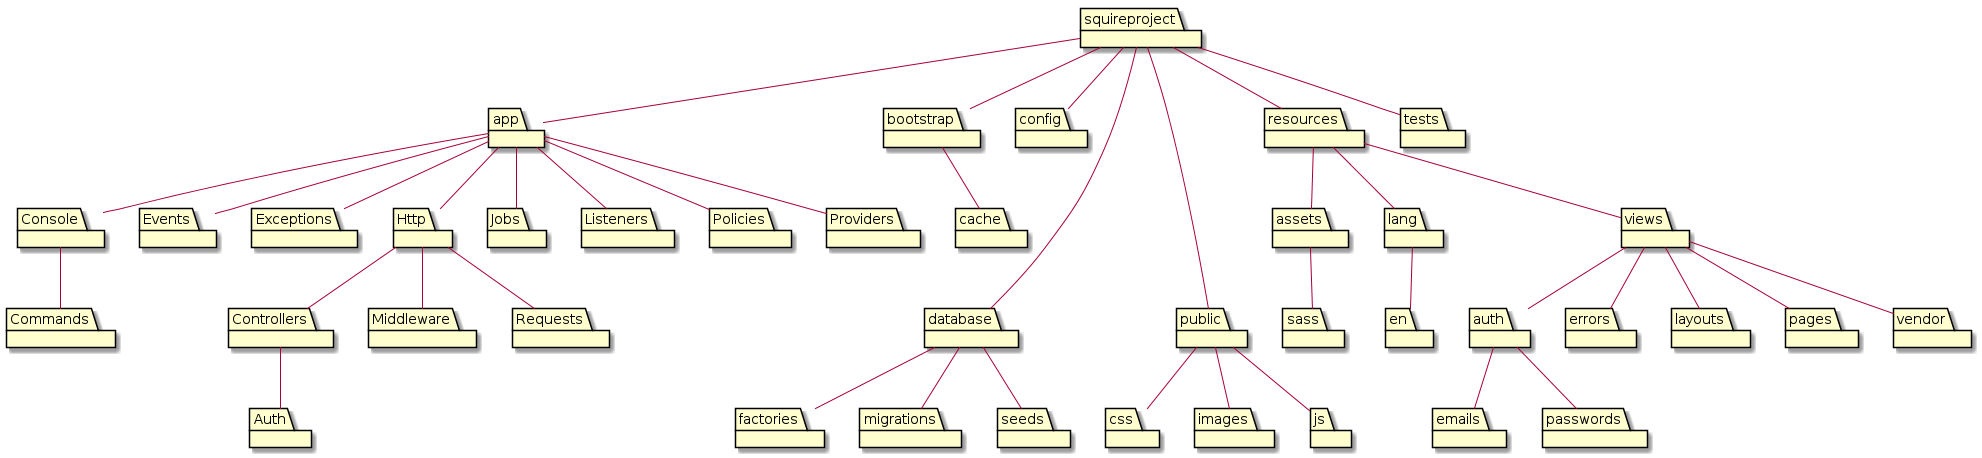
\includegraphics[width=0.9\textwidth]{diagrams/folders-overview-max}
        \end{center}
        \captionof{figure}{Squire's file structure is organized to allow for a simple and concise project flow. This structure includes seven main subfolders app, bootstrap, config, database, public, resources, and tests. Each containing crucial files allowing squireproject.com to exist.}
    \end{minipage}
    
    \begin{itemize}
        \item Main Subfolders:
        \begin{itemize}
            \item app: Contains the files that allow for the main functionality of Squire
            \item bootstrap: Contains files for configuring auto loading and for bootstrapping the framework.
            \item config: Contains project squires configuration files.
            \item database: Contains files pertaining to database migrations and seeds.
            \item public: Contains the front controller and web page assets.
            \item resources: Contains raw assets, front end views, and localization files.
            \item tests: Contains files for automated testing.
        \end{itemize}
    \end{itemize}
    
%##########################################################################################################################################################################
% app folder
%##########################################################################################################################################################################

\subsection{app folder}
\begin{itemize}
    \item Console: Artisan commands for Laravel’s built in commands.
    \begin{itemize}
        \item Commands: Contains console cammands for artisan.
        \begin{itemize}
            \item Inspire.php: 
            \item PopulateProjectsTable.php: Auto populates the mysql database \texttt{projects\_table} with some premade data.
        \end{itemize}
        \item Kernel.php: 
    \end{itemize}
    \item Events: Event classes for alerting different sub-systems to given actions.
    \item Exceptions: Exception handlers for dealing with exceptions.
    \begin{itemize}
        \item Handler.php: Exceptions that should and should not be reported.
    \end{itemize}
        \item Http: Controllers for routing data to and from squireproject.com. Middleware usable by different aspects like authentication. Requests
    \begin{itemize}
        \item Controllers: Contains all files dealing with routing data.
        \begin{itemize}
            \item Auth: Contains files dealing with authentication routing.
            \begin{itemize}
                \item AuthController.php: Routes data dealing with authentication to and from the user.
                \item PasswordController.php: Routes data pertaining to passwords from the user to the database.
            \end{itemize}
            \item Controller.php: Base class that all controllers extend for routing data.
            \item PagesController.php: Routes data dealing with html/php pages like index.blade.php, projectfinder.blade.php and etc from and to the user.
        \end{itemize}
        \item Middleware: Included software for simplifing certain tasks.
        \begin{itemize}
            \item Authenticate.php: Handles incoming authentication requests and checks if the user is autherized to see the page and if not direct them to a 401 page.
            \item EncryptCookies.php: Encrypts cookies and sets which cookies to ignore.
            \item RedirectIfAuthenticated.php: If user already authentcated then redirectes them to '/' page.
            \item VerifyCsrfToken.php: Verifies csrf tokens.
        \end{itemize}
        \item Requests: 
        \begin{itemize}
            \item Reques.php: 
        \end{itemize}
        \item Kernel.php: 
        \item routes.php: 
    \end{itemize}
    \item Jobs: Queueable jobs for Squire’s request cycle.
    \begin{itemize}
        \item Job.php: This is the base class to extend when creating new jobs.
    \end{itemize}
    \item Listeners: Handler classes for events to allow for performing actions based on triggered events.
    \item Policies: Authorization policy classes for dealing with user action.
    \item Providers: Addable 3rd-party features for extending built in features.
    \begin{itemize}
        \item AppServiceProvider.php: 
        \item AuthServiceProvider.php:
        \item EventServiceProvider.php:
        \item RouteServiceProvider.php: 
    \end{itemize}
    \item User.php: Sets variables as hidden and/or mass assignable to allow for users to have hidden passwords and grouped assignable variables.
    \item Project.php: Defines the project model that is used in the MySQL database table named projects. Allows interacting with entries from the table through PHP code.
    %\item Project.php: 
\end{itemize}

%##########################################################################################################################################################################
% bootstrap folder
%##########################################################################################################################################################################

\subsection{bootstrap folder}
\begin{itemize}
    \item cache: 
    \begin{itemize}
        \item compiled.php:
        \item services.php:
    \end{itemize}
    \item app.php: 
    \item autoload.php: 
\end{itemize}

%##########################################################################################################################################################################
% config folder
%##########################################################################################################################################################################

\subsection{config folder}
\begin{itemize}
    \item app.php: Configuration for the applications environment, debugging, localization, encryption, service providers, and etc.
    \item auth.php: Configuration for authentication options like what database users data is stored in and timeout time.
    \item broadcasting.php: Configuration for how events are broadcasted over websockets.
    \item cache.php: Configuration for cache storage settings and locations.
    \item compile.php: Configuration for custom classes artisan commands can create.
    \item database.php: Configuration for how mysql should be setup for example port number, username, password, and etc.
    \item filesystems.php: Configuration for local and cloud disk paths and settings.
    \item mail.php: Configuration for email services that should be used for example smtp, port number, username, and etc.
    \item queue.php: Configuration for Laravel's backend queue system.
    \item services.php: Configuration for storing third party service's credentials
    \item session.php: Configuration for lifetime of user sessions while idle.
    \item view.php: Configuration of paths the system should look for views (php/html pages).
\end{itemize}

%##########################################################################################################################################################################
% database folder
%##########################################################################################################################################################################

\subsection{database folder}
\begin{itemize}
    \item factories: Used primarily in unit testing, allows for entries to be made with a default set of attributes.
    \begin{itemize}
        \item ModelFactory.php:
    \end{itemize}
    \item migrations: Contains migrations for use with the Artisan migrate command. Migrations are used to create the tables in the database as well as modify their schema in the future. Also allows for rolling back of migrations to "reset" the state of the database.
    \begin{itemize}
        \item \texttt{create\_users\_table.php}:
        \item \texttt{create\_password\_resets\_table.php}:
        \item \texttt{create\_projects\_table.php}: 
    \end{itemize}
    \item seeds: Contains file used with the Artisan seeder command, allows for databases to be seeded with initial/test entries.
    \begin{itemize}
        \item DatabaseSeeder.php:
    \end{itemize}
\end{itemize}

%##########################################################################################################################################################################
% public folder
%##########################################################################################################################################################################

\subsection{public folder}
\begin{itemize}
    \item css: CSS files for html styling.
    \begin{itemize}
        \item main.css: Contains all css styling for all of squireproject.com
    \end{itemize}
    \item images: Folder for general images to be used on the site, not those for specific projects.
    \item js: Contains Javascript files.
\end{itemize}

%##########################################################################################################################################################################
% resources folder
%##########################################################################################################################################################################

\subsection{resources folder}
\begin{itemize}
    \item assets: raw assets like SASS.
    \begin{itemize}
        \item sass:
        \begin{itemize}
            \item app.scss:
        \end{itemize}
    \end{itemize}
    \item lang: setting messages and their languages used for user messages.
    \begin{itemize}
        \item en:
        \begin{itemize}
            \item auth.php:
            \item pagination.php:
            \item passwords.php: 
            \item validation.php: 
        \end{itemize}
    \end{itemize}
    \item views: front end html pages users see when viewing squireproject.com.
    \begin{itemize}
        \item auth: Contains views for authentication
        \begin{itemize}
            \item emails: Contains view for resetting password via email.
            \begin{itemize}
                \item password.blade.php:
            \end{itemize}
            \item passwords: Contains views for resetting password
            \begin{itemize}
                \item email.blade.php:
                \item reset.blade.php:
            \end{itemize}
            \item login.blade.php: View where user can login to the website.
            \item register.blade.php: View where user can register to become a part of sQuire
        \end{itemize}
        \item errors: Contains views for general errors.
        \begin{itemize}
            \item 503.blade.php: The view to show a user when they encounter a 503
        \end{itemize}
        \item layouts: Contains layouts which can be extended by other views, provides inheritance for html files.
        %\begin{itemize
         %   \item \texttt{main\_layout.blade.php}: The main layout for most pages. Includes the Header, Footer, and Nav bar. Leaves the body to be filled by its descendants.
        %\end{itemize}
        \item pages
        %\begin{itemize}
         %   \item about.blade.php: The view for the About Us page, contains information about sQuire and what it is that its trying to accomplish.
          %  \item create.blade.php: The view for the Create Project page. This page is where users can create a new project with an image, title, description, and full explanation of the projects intent.
           % \item index.blade.php: The view for the landing page for sQuire. Redirects logged in users to the Project Finder Page, otherwise pitches sQuire to the viewer and leads them to Register/Login.
            %\item project.blade.php: The view where users can see the information about a project that has already been created. Shows a picture, title, description and full explanation of the project.
            %\item projectfinder.blade.php: The view containing all the projects on squire for users to browse through. Also has a search bar to filter projec
        %\end{itemize}
        \item vendor
    \end{itemize}
\end{itemize}

%##########################################################################################################################################################################
% tests folder
%##########################################################################################################################################################################

\subsection{tests folder}
\begin{itemize}
    \item ExampleTest.php: An example test to extend from in the future.
    \item TestCase.php: The base testing case for the project.
\end{itemize}